The concept of \textcolor{ProcessBlue}{\bfseries barrier coverage} was first introduced in \cite{gage1992command} in the field of robotics. 
Up to now, barrier coverage has attracted intensive attention from research community. Earlier, almost researches focus on omni-directional sensors \cite{chen2007designing, kumar2005barrier, liu2008strong, yang2009barrier}. In \cite{kumar2005barrier}, Kumar et al. defined the concept of k-barrier coverage. Two types of barrier coverage were also introduced: weak barrier coverage and strong barrier coverage. Chen et al. \cite{chen2007designing} introduced a new model of barrier coverage called local barrier coverage. It is proved there that sensors can locally determine the existence of local barrier coverage, while it is impossible for global barrier coverage. Under this model, the authors developed a sleep-wakeup algorithm for maximizing the network lifetime and showed that their algorithm can provide close to optimal enhancement. In \cite{liu2008strong}, Liu et al. derived critical conditions for strong barrier coverage in two-dimensional rectangular where sensors are deployed uniformly and randomly. They pointed out that if width $W$ and length $L$ of the rectangular satisfies $W=\Omega(L)$, there exist, with high probability, multiple disjoint barriers when sensors density reaches a certain value. Whereas, when $W=O(L)$, with high probability, there will be a crossing path not covered by any sensor regardless of the sensor density. Based on this result, the authors devised an efficient distributed algorithm to construct disjoint barriers in a large sensor network to cover long boundary areas of irregular shapes. In \cite{yang2009barrier}, based on probabilistic sensing model, Yang et al. studied barrier coverage problem under the assumption that neighboring sensors may collaborate with each other to form a virtual sensor which makes the detection decision depending on combined sensed readings. This is referred to as barrier information coverage.\par
Later, with the wide use of directional sensor, especially camera sensor, there were more and more interest in Wireless Camera Sensor Networks (WCSNs). Barrier coverage problems in WCSNs are much more difficult and challenging compared to those in traditional scalar WSNs. The biggest difference between WCSNs and scalar WSNs and also the biggest challenge when working with WCSNs is the directional characteristic of camera sensor. Since directionality was taken into consideration, many coverage models have been proposed for improving monitoring performance of sensor networks. \par
In this paper, we study ($k-\omega$) coverage model. In the followings, we present some related works studying on some different coverage models which are closely relevant to ($k-\omega$) coverage model as well as previous works on ($k-\omega$) coverage model. \par
In order to get more information of the object, especially face regconition, full-view coverage was introduced in \cite{wang2011full} by Wand and Cao. An object is full-view covered if there is always a camera to cover it no matter which direction it faces and the angle between the camera’s viewing direction and the object’s facing direction is less than a predefined parameter $\theta$.
The authors proposed a method for full-view coverage verification on a target field. After that, they derived an estimation of the sensor density needed for full-view coverage in a random deployment. Based on this work, the authors further studied the problem of constructing a camera barrier in \cite{wang2011barrier}. They proposed a method to select camera sensors from an arbitrary deployment to form a camera barrier and then presented a technique for reducing the number of cameras used since there might be redundant cameras (cameras that can be turned off without breaking the barrier) after barrier is formed. The monitoring region is divided into sub regions where each sub region is a set of points covered by the same set of sensors. Using notion of safe region, the authors can verify whether or not a sub region is full-view covered. After that, they can transform the problem into graph and finding a barrier is converted to finding a path from source node to sink node in the graph. For redundancy reduction, another type of graph is introduced and the problem is equivalent to maximum independent vertex set problem. \par
Inspired by this work, in \cite{ma2012minimum}, Ma et al. proposed a better method for constructing camera barrier. The authors proved that for a sub region which is not full-view covered, it always contains two parts: the full-view covered one and the non full-view covered one. Then, each node in the graph can be a full-view covered sub region or the full-view covered part of a sub region that is not full-view covered. The problem of finding the minimum camera barrier is transformed to the problem of finding the shortest path from source node to sink node in the graph. \textcolor{ProcessBlue}{\bfseries However, we see that the algorithm used in this work cannot be used to solve the problem}. This algorithm can be considered as a variant of Dijkstra algorithm. The only two differences are: (1) the edge has no weight but each vertex $v$ has a "weight" denoted by $I(v)$ and (2) the operator used for updating label of a vertex is union instead of addition. The second difference is the reason why the algorithm has prolem. According to the algorithm, when a vertex $v$ is labeled, every previous vertex in the path from source vertex $s$ to $v$ is also labeled. Supposed $u$ is such a vertex between $s$ and $v$, the shortest path from $s$ to $u$ must be contained in the path from $s$ to $v$. But this is not true when the operator union is used (figure \ref{fig:01})
\begin{figure}[p]
	\centering
	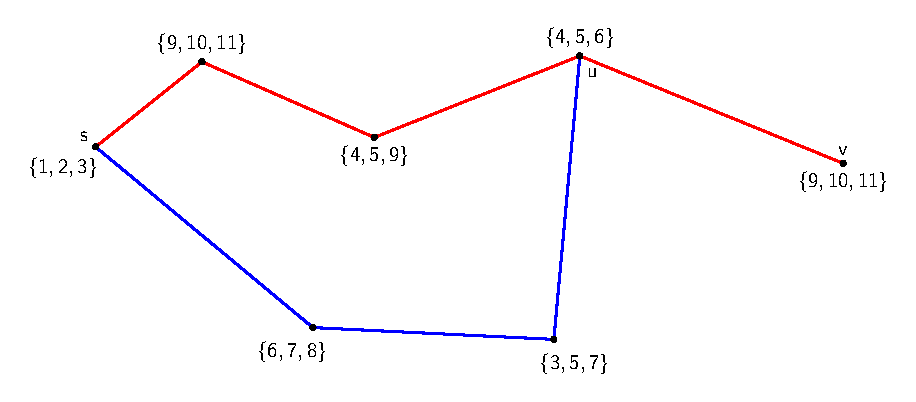
\includegraphics[scale=1.]{wrongDijstra.pdf}
	\caption{Red line is shortest path from $s$ to $v$. Blue line is shortest path from $s$ to $u$}
	\label{fig:01}
\end{figure}

Following the above studies, there have been much effort on various problems under full-view coverage model. In \cite{manoufali2016effect}, the authors study the effects of realistic sea surface movements in achieving full-view coverage in CSN. They also addressed the problem of reducing the total transmission power among sensors by proposing a cooperative transmission method. Under the deterministic deployment strategy, the authors in \cite{wu2017node} proposed an efficient deployment pattern algorithm DPA to compute the critical density and positions of sensors for achieving full-view coverage on the target field. Moreover, they devised a local neighboring-optimal selection algorithm (LNSA) to find a minimum set of camera nodes guaranteeing the region of interest (ROI) can be full-view covered and schedule camera nodes into sleeping or working mode. In \cite{liu2018full}, Liu et al. studied full-view barrier coverage problem in mobile CSN. They defined full-view coverage model of mobile camera sensors. Based on this model, they divided the target field into some connected grids and used these grids to construct a weighted directed graph. The problem of building a full-view barrier with minimum number of sensors was then converted to the problem of finding the shortest path in the constructed graph by using Dijkstra algorithm.\par
	
Motivated by the purpose of monitoring the object from multiple perspectives, in \cite{tseng2012k}, Tseng et al. introduced the notion of $k$-angle coverage. To avoid duplicating information from multiple sensors simultaneously monitoring an object, an angle constraint was added, which guaranteed two sensors cannot appear in an angle range of $\omega$ around the object (figure \ref{fig:02}). With this constraint, the notion of $k-\omega-$angle coverage was defined. It was pointed out that if an object is $k-\omega-$angle covered, there is no angle larger than $2\pi-(k-1)\omega$ of the object that is not covered by any sensor. This means that an object that is $k-\omega-$angle covered is also full-view covered with parameter $\theta=\displaystyle\frac{2\pi-(k-1)\omega}{2}$. Hence, $k-\omega-$angle coverage can be considered as a special case of full-view coverage with the number of camera sensors covering the object is fixed. Under this new coverage model, the paper focused on addressing the problem of $k-\omega-$angle covering maximum number of objects using minimum number of sensors. The sensors can rotate around its location but cannot move. The authors proved that there have only finite possibilities that a sensor can rotate to achieve optimal coverage. Then, a greedy scheme was proposed to gradually turn each sensor into fixed position. Finally, all redundant sensors were set to low-power mode to save energy and optimize network performance.
\begin{figure}[p]
	\centering
	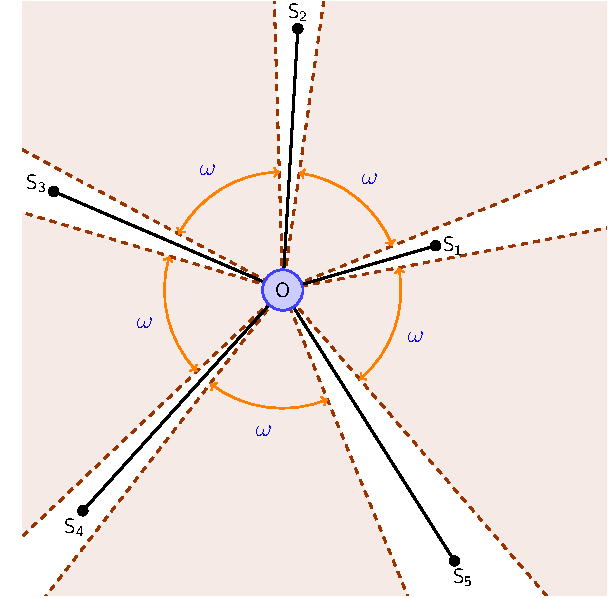
\includegraphics[scale=.7]{komega.pdf}
	\caption{$O$ is 5-$\omega$-angle covered by $\{S_1, S_2, S_3, S_4, S_5\}$}
	\label{fig:02}
\end{figure}

In \cite{xu2016minimum}, the authors studied the problem of constructing k-$\omega$-angle barrier using minimum number of sensors, which is referred to as minimum k-$\omega$-angle barrier coverage problem (MkABC). The paper presented MkABC problem in two deployment scheme. Under deterministic deployment, a geometric method was proposed, which used the feature of regular polygon to construct a ($k-\displaystyle\frac{\pi}{k}$)-angle barrier. When sensors are randomly deployed in the monitoring region, the MkABC becomes more difficult. In this scenario, the authors proposed a grid-based method, where each grid is judged to be ($k-\omega$)-angle covered or not. MkABC problem is then transformed to finding shortest path in graph. The algorithm used is the same as one used in \cite{ma2012minimum}, which has some problems as aforementioned. Besides, the accuracy level and computational cost of this method as well as generic grid-based method depends on grid size. The decreasing in grid size leads to increasing in both computational cost and accuracy level, which is not expected. There must be a trade-off between these two factors. \par

So far, we have discussed different types of barrier coverage such as: weak/strong barrier coverage, k-barrier coverage, full-view camera barrier, k-$\omega$-angle camera barrier. Most of the existing works in barrier coverage focused on two main problems: (1) achieving barrier coverage, which answer the question whether a sensors deployment forming a barrier in the monitoring region and (2) minimize the number of sensors using to construct a barrier. Chen et al. \cite{chen2008measuring} first mentioned the problem of measuring the quality of barrier coverage. According to that, just consider whether or not a sensor network providing barrier coverage, which is equivalent to measuring its quality as either 0 or 1, is not enough since there might be many different levels of quality. Using the notion of $L$-local $k$-barrier coverage, the authors proposed to measure the quality of $k$-barrier coverage for a belt region as the maximum value of $L$ that the belt is $L$-local $k$-barrier covered. A belt region is said to be $L$-local $k$-barrier covered if every zone of length $L$ in the region is $k$-barrier covered. Two other metrics that they had considered are: (1) the number of sensors needed to make the belt k-barrier covered and (2) the probability that an intruder following a randomly picked path being detected by at least k sensors. All these three metrics can effectively measure the coverage quality, however, they always provide the same result when sensor network has already achieved k-barrier coverage, i.e, the probability of detecting the intruder by $k$ sensors is always 100\%.\par

In this paper, we investigate the $A(k-\omega)ABC$ problem. After considering many related works, we see that previous approaches to $A(k-\omega)ABC$ problem are not yet efficient and there are rooms for improvement. Therefore, we proposed a grid-based method called \textcolor{ProcessBlue}{\bfseries Dynamic Partition} to solve this problem. Furthermore, we want to measure the quality of object's information recorded by sensors network when it crosses the barrier. Since the metrics proposed in \cite{chen2008measuring} is for $k$-barrier coverage model, it cannot apply to our ($k-\omega$) coverage model. Moreover, this metrics only works when sensors network has not provided $k$-barrier coverage yet. In contrast, we need a metrics for measuring quality of the ($k-\omega$) barrier, which means the barrier must have been already constructed. These prompts us to come up with a new metrics called \textcolor{ProcessBlue}{\bfseries Differentiation Exposure}.
